\documentclass[border = 5pt, tikz]{standalone}

\begin{document}
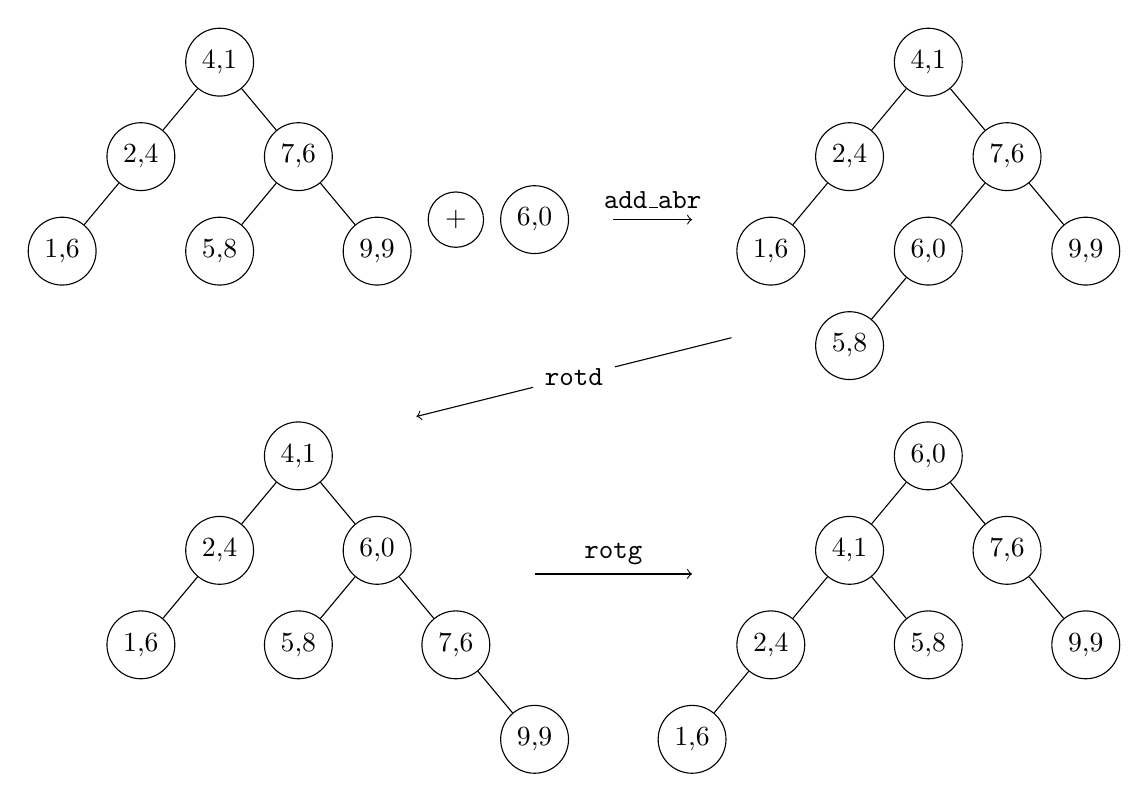
\begin{tikzpicture}[
  every node/.style = {minimum width = 2em, draw, circle},
  level 1/.style = {sibling distance = 20mm, level distance = 12mm},
  level 2/.style = {sibling distance = 20mm, level distance = 12mm}
  ]
  %first tree
  \node {4,1}
  child {node {2,4}
        child {node {1,6}}
        child {edge from parent[draw = none]}
  }
  child {node {7,6}
        child {node {5,8}}
        child {node {9,9}}
  };

  \begin{scope}[xshift=3cm, yshift=-2cm]
    \node {+};
  \end{scope}

  \begin{scope}[xshift=4cm, yshift=-2cm]
    \node {6,0};
  \end{scope}

  %second tree
  \begin{scope}[xshift=9cm]
    \node {4,1}
  child {node {2,4}
        child {node {1,6}}
        child {edge from parent[draw = none]}
  }
  child {node {7,6}
        child {node {6,0}
                child {node {5,8}}
                child {edge from parent[draw = none]}}
        child {node {9,9}}
  };
  \end{scope}

  %third tree
  \begin{scope}[xshift=1cm, yshift=-5cm]
    \node {4,1}
  child {node {2,4}
        child {node {1,6}}
        child {edge from parent[draw = none]}
  }
  child {node {6,0}
        child {node {5,8}}
        child {node {7,6}
            child {edge from parent[draw = none]}
            child {node{9,9}}
        }
  };
  \end{scope}

  %fourth tree
  \begin{scope}[xshift=9cm, yshift=-5cm]
    \node {6,0}
  child {node {4,1}
        child {node {2,4}
                child {node {1,6}}
                child {edge from parent[draw = none]}}
        child {node {5,8}}
  }
  child {node {7,6}
            child {edge from parent[draw = none]}
            child {node {9,9}}
  };
  \end{scope}

  \draw[-to] (5,-2) -- (6,-2);
  \node[draw = none] at (5.5,-1.75) {\texttt{add\_abr}};
  \draw[-to] (6.5,-3.5) -- (2.5,-4.5);
  \node[draw = none, fill=white] at (4.5,-4) {\texttt{rotd}};
  \draw[-to] (4,-6.5) -- (6,-6.5);
  \node[draw = none] at (5, -6.25) {\texttt{rotg}};
\end{tikzpicture}
\end{document}
